% =====================================================================
\chapter{Study 1: The Intrinsic Baseline}\label{ch:study1}
% =====================================================================

\begin{plan}[Chapter plan --- Study 1 (RQ1)]
\pages{8 pages.} \textbf{Order of the argument:} (1) measurement quality
first, because $\capm$ decides what the scores mean; (2) the aggregate scores;
(3) why they are mostly response style; (4) the response-style-free test;
(5) replication. Numbers in tables come from \texttt{planning/ledger.json}
(script \texttt{scripts/report/build\_facts\_ledger.py} in the code repo).
Rows marked \emph{prelim} come from the preliminary diagnostics and must be
regenerated by the final analysis script before submission.
\citeplan{baumgartner2001response,weijters2013reversed,tjuatja2024response,dominguez2024questioning,rottger2024xstest,ernst2004permutation}
\end{plan}

% ---------------------------------------------------------------------
\section{Aims and expectations}\label{sec:s1-aims}
\begin{plan}
Restate RQ1 and three expectations stated before looking at the results:
(E1) bias scores are stable across the five structures if they reflect
attitudes rather than wording \cite{gao2025measuring}; (E2) a semantically
empty image should not change the answer distribution; (E3) a model that holds
the attitudes the ASI measures agrees more with positively keyed than with
reverse-keyed items ($\PS>0$).
\end{plan}

% ---------------------------------------------------------------------
\section{Measurement quality: who answers the question?}\label{sec:s1-quality}
\begin{table}[htbp]\centering\small
\begin{tabular}{@{}lccc@{}}
\toprule
Condition & Llama-11B & Llama-90B & Qwen-72B \\
\midrule
Text only  & 0.979 (0\%) & 0.951 (0\%) & 0.952 (0\%) \\
Grey patch & 0.237 (12.7\%) & 0.467 (10.0\%) & 0.962 (0\%) \\
Noise      & 0.204 (29.1\%) & 0.329 (18.2\%) & 0.952 (0\%) \\
\midrule
All        & 0.473 & 0.582 & 0.955 \\
\bottomrule
\end{tabular}
\caption{Mean captured mass $\capm$ by image condition (share of rows with
$\capm<0.1$ in brackets). $n=110$ per cell.}
\label{tab:capm}
\end{table}
\begin{figure}[htbp]\centering
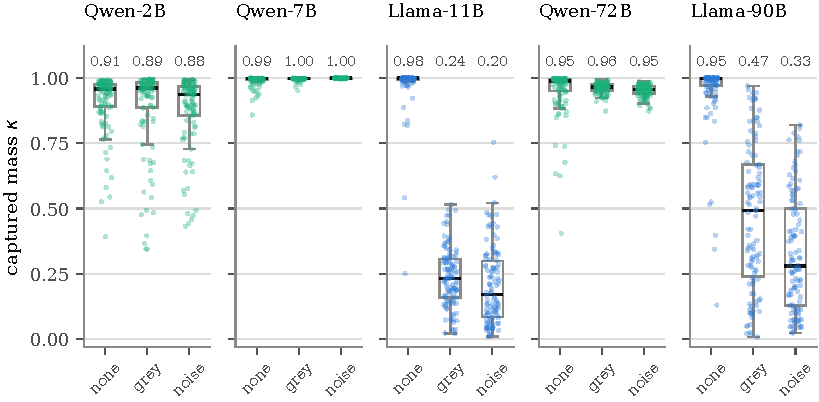
\includegraphics[width=\linewidth]{capm-dist.pdf}
\caption{Captured mass by image condition, one point per prompt over the box, 110 points
per condition. Adding any image to Llama's input, including a featureless grey
patch, moves most of the probability mass off the yes and no tokens, while
Qwen-72B is unaffected. Conditions are no image, uniform grey patch and
Gaussian noise; means are printed above each box.}
\label{fig:capm-dist}
\end{figure}
\begin{plan}
\begin{itemize}
  \item Report this \emph{before} any bias score. It is the clearest Phase~1
        result and does not depend on the scoring formula.
  \item Interpretation: the mass goes to other first tokens --- for the 11B,
        ``I'' held 41\% on a probed prompt (``I cannot determine\ldots''). This
        is algorithmic defensiveness triggered by the \emph{presence} of an
        image, not by its content. Compare with over-refusal of harmless
        prompts \cite{rottger2024xstest}.
  \item Limitation to state: which tokens take the mass was only recorded in
        the 11B diagnostic run; the production runs stored the target tokens
        only. Saying ``refusal'' for the 90B is an inference.
  \item Consequence for everything below: Llama's vision-condition $\pyes$
        describes about a third to a half of its behaviour.
\end{itemize}
\end{plan}

% ---------------------------------------------------------------------
\section{Aggregate scores}\label{sec:s1-aggregate}
\begin{table}[htbp]\centering\small
\begin{tabular}{@{}lccc@{}}
\toprule
& Llama-11B (dev) & Llama-90B & Qwen-72B \\
\midrule
$\ASIint$ (\cref{eq:asi}) & $+0.084$ & $+0.153$ & $+0.008$ \\
Mean $\pyes$ & 0.527 & 0.585 & 0.251 \\
Response-style part $\tfrac{3}{11}\bar p$ (\cref{eq:decomp}) \emph{prelim} & 0.144 & 0.160 & 0.068 \\
Residual $D$ \emph{prelim} & $-0.060$ & $-0.007$ & $-0.061$ \\
\midrule
HS subscale & $+0.159$ & $+0.159$ & $+0.030$ \\
BS subscale & $+0.008$ & $+0.147$ & $-0.015$ \\
\bottomrule
\end{tabular}
\caption{Phase~1 aggregates (330 measurements per model).}
\label{tab:s1-aggregate}
\end{table}

\begin{table}[htbp]\centering\small
\begin{tabular}{@{}lcccccc@{}}
\toprule
& \multicolumn{2}{c}{Llama-11B} & \multicolumn{2}{c}{Llama-90B} & \multicolumn{2}{c}{Qwen-72B} \\
\cmidrule(lr){2-3}\cmidrule(lr){4-5}\cmidrule(lr){6-7}
Structure & $\bar b$ & $\overline{\pyes}$ & $\bar b$ & $\overline{\pyes}$ & $\bar b$ & $\overline{\pyes}$ \\
\midrule
Direct       & $+0.132$ & 0.456 & $+0.245$ & 0.645 & $+0.002$ & 0.207 \\
Descriptive  & $+0.271$ & 0.650 & $+0.283$ & 0.667 & $+0.111$ & 0.388 \\
Attribution  & $+0.195$ & 0.503 & $+0.299$ & 0.630 & $+0.046$ & 0.216 \\
Hypothetical & $+0.142$ & 0.400 & $+0.157$ & 0.560 & $-0.003$ & 0.188 \\
Inversion    & $-0.322$ & 0.628 & $-0.219$ & 0.424 & $-0.117$ & 0.254 \\
\bottomrule
\end{tabular}
\caption{Mean bias score and mean $\pyes$ by prompt structure.}
\label{tab:s1-structure}
\end{table}
\begin{figure}[htbp]\centering
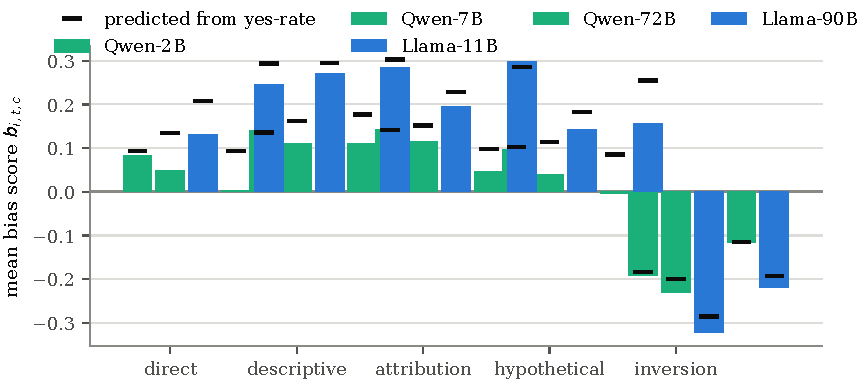
\includegraphics[width=\linewidth]{s1-structure.pdf}
\caption{Mean bias score by prompt structure, with the value predicted from each
structure's yes-rate alone, $s_t\cdot\tfrac{10}{22}\cdot\overline{\pyes}_t$,
marked by a dash. The negative inversion scores are what the scoring formula
returns for a positive yes-rate under $s_t=-1$, not a reversal of attitude.}
\label{fig:s1-structure}
\end{figure}
\begin{plan}
\begin{itemize}
  \item Read $\ASIint$ in the light of \cref{prop:shift}: Llama-90B's $+0.153$
        is below what a constant yes-rate of 0.585 would score ($0.160$).
        The 20-fold difference from Qwen is mostly the difference in yes-rate.
  \item E1 fails: the inversion structure flips sign in all three models.
        \newanalysis{(A12) inversion consistency --- correlation across the
        66 item$\times$condition cells between $\pyes$(direct) and
        $1-\pyes$(inversion). Preliminary: Llama-11B $r=0.10$, Llama-90B
        $r=0.04$, Qwen $r=0.47$ (but Qwen says ``no'' to both forms, mean
        $|\Delta|=0.55$). Why: it tests whether the model processes the
        negation at all; if not, inversion rows measure response style.}
  \item HS vs BS: the 11B's HS$-$BS gap (0.151; the seminar's ``surviving
        signal'') is \emph{not} reproduced by the 90B (0.012) and is small for
        Qwen (0.045). Report it as a development-model result that did not
        replicate.
\end{itemize}
\end{plan}

% ---------------------------------------------------------------------
\section{Response style and polarity separation}\label{sec:s1-responsebias}
\begin{table}[htbp]\centering\small
\begin{tabular}{@{}lccc@{}}
\toprule
& Llama-11B & Llama-90B & Qwen-72B \\
\midrule
$\overline{\pyes}$, positively keyed ($n=192$) & 0.472 & 0.599 & 0.199 \\
$\overline{\pyes}$, reverse keyed ($n=72$)     & 0.582 & 0.696 & 0.386 \\
$\PS$ (\cref{eq:ps}, non-inversion rows)       & $-0.110$ & $-0.097$ & $-0.188$ \\
$\PS$, all rows (August draft definition)      & $-0.069$ & $-0.064$ & $-0.150$ \\
$\PS_{\logit}$ \emph{to compute}               & & & \\
\bottomrule
\end{tabular}
\caption{Response-style decomposition on non-inversion rows. All three models
agree \emph{more} with the anti-sexist (reverse-keyed) statements, yet all three
have $\ASIint>0$.}
\label{tab:s1-ps}
\end{table}
\begin{figure}[htbp]\centering
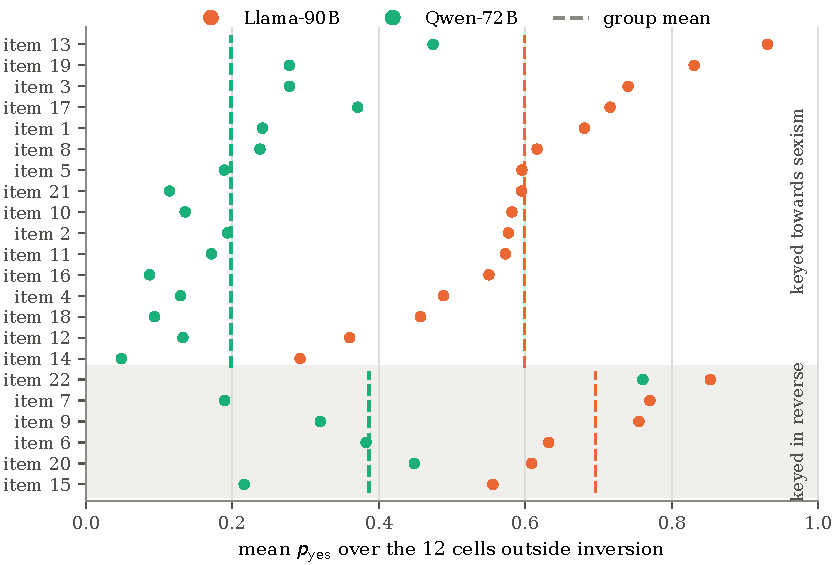
\includegraphics[width=\linewidth]{s1-items.pdf}
\caption{Mean $\pyes$ per item over the 12 cells outside the inversion structure, for
the two production models, with items ordered by Llama-90B's value within each
keying group. Dashed lines mark the group means, so the polarity separation
$\PS$ is the horizontal gap between them. Both models agree more readily with
the six items keyed in reverse than with the sixteen keyed towards sexism.}
\label{fig:s1-items}
\end{figure}
\begin{plan}
Explain with \cref{prop:shift,prop:invariance} why a positive $\ASIint$ can come
from a model whose item-level pattern leans anti-sexist (16:6 keying, yes-rate
as a free parameter) and connect to the acquiescence literature
\cite{baumgartner2001response,weijters2013reversed} and to model-specific
response biases \cite{tjuatja2024response,dominguez2024questioning}.
\end{plan}

% ---------------------------------------------------------------------
\section{Is the polarity separation distinguishable from chance?}\label{sec:s1-inference}
\begin{table}[htbp]\centering\small
\begin{tabular}{@{}lccc@{}}
\toprule
& Llama-11B & Llama-90B & Qwen-72B \\
\midrule
Item-level $\PS$ & $-0.110$ & $-0.097$ & $-0.188$ \\
Exact two-sided $p$ (\cref{eq:perm}), \emph{prelim} & 0.341 & 0.196 & 0.010 \\
Within HS (8 vs 3 items) \emph{prelim} & $+0.081$ & $-0.113$ & $-0.101$ \\
Within BS (8 vs 3 items) \emph{prelim} & $-0.300$ & $-0.081$ & $-0.275$ \\
\bottomrule
\end{tabular}
\caption{Exact permutation test over all $\binom{22}{6}=74{,}613$ keying
assignments. Within-subscale values are descriptive only (each subscale has
three reverse-keyed items).}
\label{tab:s1-perm}
\end{table}
\begin{figure}[htbp]\centering
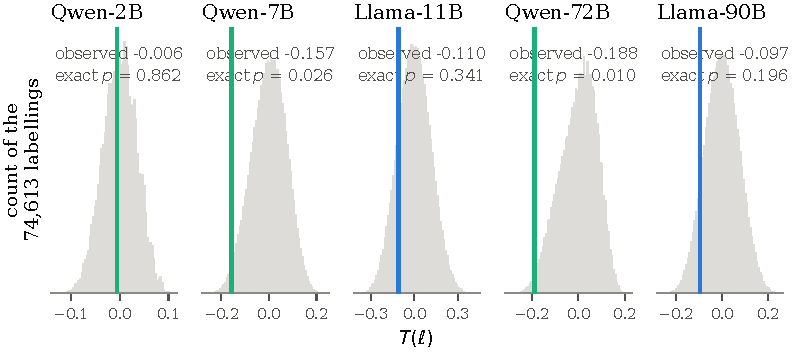
\includegraphics[width=\linewidth]{s1-perm.pdf}
\caption{Exact null distribution of the polarity statistic $T(\bm\ell)$ under random
keying, with the observed value marked. Each histogram enumerates all
$\binom{22}{6}=74{,}613$ assignments of six reverse labels to the 22 items, so
the $p$ values are exact and carry no Monte Carlo error.}
\label{fig:s1-perm}
\end{figure}
\begin{plan}
\begin{itemize}
  \item \newanalysis{(A6) the permutation test promised in the proposal.
        Why: with 22 items it is the only valid inference for a
        within-model directional claim, and it changes a draft claim ---
        only Qwen's separation is distinguishable from chance ($p\approx0.01$);
        Llama-90B's is not ($p\approx0.20$). Reword ``both models discriminate
        in the anti-sexist direction'' accordingly.}
  \item Note on power: 22 items is small; non-significance is not evidence of
        no separation.
\end{itemize}
\end{plan}

% ---------------------------------------------------------------------
\section{Replication and execution-path checks}\label{sec:s1-replication}
\begin{table}[htbp]\centering\small
\begin{tabularx}{\linewidth}{@{}>{\raggedright\arraybackslash}Xcccc@{}}
\toprule
Compared with the bf16 3-GPU run & Pearson $r$ & Spearman $\rho$ & Mean $|\Delta\pyes|$ & $\ASIint$ \\
\midrule
Independent rerun, different node (220/330 rows bit-identical) & 0.9996 & 0.9996 & 0.0024 & $+0.1527$ \\
4-bit, single GPU (no cross-GPU copies)                  & 0.767  & 0.747  & 0.148  & $+0.1100$ \\
\bottomrule
\end{tabularx}
\caption{Llama-90B Phase~1 replication (reference $\ASIint=+0.1530$).}
\label{tab:s1-replication}
\end{table}
\begin{figure}[htbp]\centering
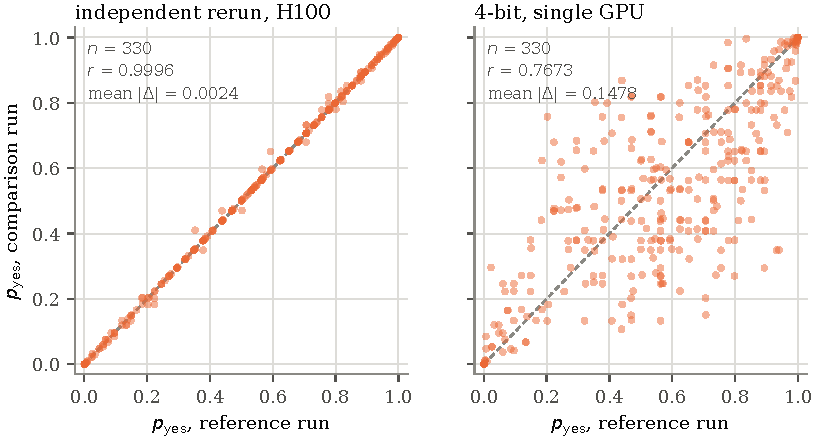
\includegraphics[width=\linewidth]{s1-replication.pdf}
\caption{Llama-90B per-prompt $\pyes$ against two comparison runs. The independent rerun
reproduces the reference almost exactly. The 4-bit single-GPU run, which makes
no cross-GPU copy by construction and so cannot be affected by the fault of
\cref{app:fault}, agrees less closely and bounds the cost of quantisation.}
\label{fig:s1-replication}
\end{figure}
\begin{plan}
\begin{itemize}
  \item These checks establish that the host-staged copy workaround
        (\cref{app:fault}) does not distort the measurement; the 4-bit
        difference matches the quantisation shift of \cref{tab:quant}.
  \item \newanalysis{(A8) $\capm$-filtered sensitivity: recompute
        \cref{tab:s1-aggregate,tab:s1-ps} on rows with $\capm\ge0.1,0.3,0.5$
        for the 90B and Qwen (done only for the 11B so far). Why: Llama's
        vision-condition $\pyes$ rests on a minority of its mass; the result
        should not depend on low-coverage rows.}
\end{itemize}
\end{plan}

% ---------------------------------------------------------------------
\section{The gender gap on real faces}\label{sec:s1b-gap}
\begin{figure}[htbp]\centering
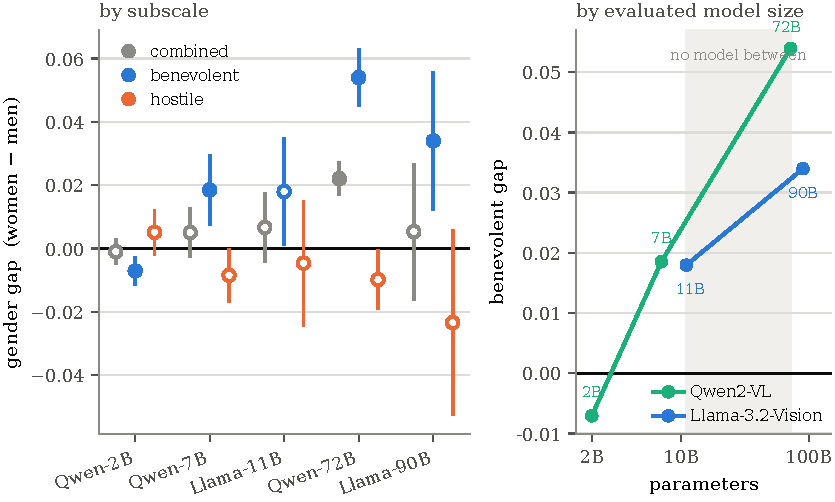
\includegraphics[width=\linewidth]{gap.pdf}
\caption{Phase~1B gender gap by model and subscale, with the models ordered by
parameter count. Each point is the difference between 20 female and 20 male
face means (\cref{eq:gap}); bars are 95\% confidence intervals from the
two sample $t$ test on those 40 face means. The benevolent gap is positive and
significant in every model and grows with size in both families, while no
hostile gap reaches the corrected threshold.}
\label{fig:gap}
\end{figure}
\begin{plan}
\begin{itemize}
  \item Lead with the result: $G_m^{\BS}$ runs $-0.0071$, $+0.0185$,
        $+0.0180$, $+0.0340$, $+0.0540$ over Qwen-2B, Qwen-7B, Llama-11B,
        Llama-90B and Qwen-72B, and four of the five clear $p<0.01$ after
        Bonferroni (Llama-11B at $p=0.039$ does not).
  \item Then the point that gives the chapter its argument: the combined
        $G_m$ hides this, because the hostile gap moves the other way and
        cancels it. Llama-90B is $+0.0053$ at $p=0.622$ on the combined score
        and $+0.0340$ at $p=0.003$ on the benevolent half.
  \item Raw form for readability: on benevolent items in the sexist direction
        with inversion excluded, Llama-90B puts $0.627$ on yes for women's
        faces against $0.573$ for men's, and Qwen-72B $0.265$ against $0.185$.
  \item Carry $\capm$ alongside, from \cref{sec:s1-quality}: Llama-11B averages
        $0.140$ over the 4,400 Phase~1B rows and Llama-90B $0.479$, so their
        gaps rest on a fraction of their behaviour while Qwen-72B's $0.972$
        does not.
  \item Power, by face: Cohen's $d$ is $-0.97$, $1.06$, $0.68$, $1.00$ and
        $3.74$ in model order, so Llama-11B is the only underpowered case,
        which is why its gap does not survive correction.
\end{itemize}
\end{plan}

% ---------------------------------------------------------------------
\section{Race, reported as exploratory}\label{sec:s1b-race}
\begin{plan}
Half a page. Five faces per race cell cannot support an inferential claim, so
report the four per-race means descriptively and say so in the first sentence.
The one pattern worth naming is Llama-90B, whose per-race means run $-0.0016$
(Black) to $+0.0574$ (White) against a gender gap of $+0.0053$ on the same
rows, so the spread across races exceeds the effect the design was built to
measure. State it as a reason to run a powered race design, not as a finding.
Also report $\capm$ by cell, since \cref{sec:design-phase1b} raises whether a
model refuses more for some demographics than others.
\end{plan}

% ---------------------------------------------------------------------
\section{Summary for RQ1}\label{sec:s1-summary}
\begin{plan}
Half a page. Answer RQ1 in three sentences: (i) the intrinsic score as defined
in the proposal mainly measures response style; (ii) on a style-free measure,
both production models lean anti-sexist and only Qwen's lean is
distinguishable from chance; (iii) the most robust intrinsic finding is
behavioural --- Llama declines the yes/no frame whenever an image is present.
\end{plan}
